% vim : foldmethod=marker
\documentclass[a4paper,12pt]{book}

\usepackage{styleperso}
\usepackage{todonotes}

\setuptodonotes{inline, color=blue!30}
% \setlength{\marginparwidth}{2.0cm}
% \bibliography{/home/webersa/Documents/Articles/biblatex.bib}

% =====================================================================================
% ========== Bibliography {{{
\bibliography{/home/samuel/Documents/IGE/Articles/biblatex.bib}
% }}}
% =====================================================================================

% =====================================================================================
% ============= BOOK MARK {{{
% \bookmarksetup{color=blue}
% \bookmark[page=1,level=0]{Sample document}
% }}}
% =====================================================================================

% =====================================================================================
% ========= New command {{{
\DeclareMathOperator*{\argmin}{arg\,min} % thin space, limits underneath in displays
\newcolumntype{P}[1]{>{\centering\arraybackslash}m{#1}}
\renewcommand{\hat}{\widehat}

\newcommand{\E}[1]{\cdot 10^{#1}}
\newcommand{\NOt}{\ce{NO3^-}}
\newcommand{\SOq}{\ce{SO4^2-}}
\newcommand{\NHt}{\ce{NH3}}
\newcommand{\NHq}{\ce{NH4^+}}
\newcommand{\NA}{\ce{NO3NH4}}
\newcommand{\SA}{\ce{SO4(NH4)2}}
\newcommand{\OP}{\text{OP}}
\newcommand{\PM}{\text{PM}}
\newcommand{\PMdix}{\ce{PM10}}
\newcommand{\PMdc}{\ce{PM_{2.5}}}
\newcommand{\PMun}{\ce{PM1}}
\newcommand{\OPm}{\texorpdfstring{\text{OP\textsubscript{m}}}{OPm}}
\newcommand{\OPv}{\texorpdfstring{\text{OP\textsubscript{v}}}{OPv}}
\newcommand{\POm}{\texorpdfstring{\text{PO\textsubscript{m}}}{POm}}
\newcommand{\POv}{\texorpdfstring{\text{PO\textsubscript{v}}}{POv}}
\newcommand{\OPDTT}{\text{OP}$^\text{DTT}$}
\newcommand{\OPDTTv}{\text{OP}$^\text{DTT}_\text{v}$}
\newcommand{\OPDTTm}{\text{OP}$^\text{DTT}_\text{m}$}
\newcommand{\OPAA}{\text{OP}$^\text{AA}$}
\newcommand{\OPAAv}{\text{OP}$^\text{AA}_\text{v}$}
\newcommand{\OPAAm}{\text{OP}$^\text{AA}_\text{m}$}
\newcommand{\PODTT}{\text{PO}$^\text{DTT}$}
\newcommand{\PODTTv}{\text{PO}$^\text{DTT}_\text{v}$}
\newcommand{\PODTTm}{\text{PO}$^\text{DTT}_\text{m}$}
\newcommand{\POAA}{\text{PO}$^\text{AA}$}
\newcommand{\POAAv}{\text{PO}$^\text{AA}_\text{v}$}
\newcommand{\POAAm}{\text{PO}$^\text{AA}_\text{m}$}
\newcommand{\BCwb}{BC\textsubscript{wb}}
\newcommand{\BCff}{BC\textsubscript{ff}}
\newcommand{\Xg}{{\mathbf{X}^{-g}}}
\newcommand{\OMEGA}{\mathbf{\Omega}}

% }}}
% =====================================================================================



\graphicspath{{figures/}}

% =====================================================================================
% ==== Title page {{{
\author{Samuël Weber}
\title{Aerosols sources and their contribution to the oxidative potential of Particulate Matter}
% }}}
% =====================================================================================

\begin{document}


% % \Sethpageshift{26mm}  %%optionnel : à décommenter si besoin pour ajout d'espace afin de center la couvérture horizontalement (valeur par défaut est -5.5mm)
\Sethpageshift{0mm}     %%optionnel : à décommenter si besoin pour ajout d'espace afin de center la couvérture horizontalement (valeur par défaut est -5.5mm)
\Setvpageshift{-19mm}   %%optionnel : à décommenter si besoin pour ajout d'espace afin de center la couvérture verticalement (valeur par défaut est -15.5mm)
%\Universite{}    %%optionnel : à décommenter et à renseigenr si vous voulez changer le non d'université
%\Grade{}         %%optionnel : à décommenter et à renseigenr si vous voulez changer le grade

\Specialite{Océan, Atmosphère, Hydrologie}
\Arrete{25 mai 2016}
\Auteur{Samuël Weber}
\Directeur{Jean-Luc \bsc{Jaffrezo}}
\CoDirecteur{Gaëlle \bsc{Uzu}}    %%optionnel : à décommenter et à renseigenr si présence d'un Co-directeur de thèse
\Laboratoire{Institut des Géosciences de l'Environnement}
\EcoleDoctorale{Terre Univers Environnement}
\Titre{Contribution des sources d'aérosols au potentiel oxydant}
% \TitreEN{On the source of the oxydizing potential of aerosols}
\Soustitre{vers une meilleure prise en compte de la qualité de l'air}      %%optionnel : à décommenter et à renseigenr si présence d'un sous-titre de thèse
\Depot{to be determined (normalement 20 octobre 2020)}
% Commande pour création de nouvelles catégories dans le jury:
%\UGTNewJuryCategory{...NomDeLaCategorie...}{...Definition...}
% Exemple \UGTNewJuryCategory{UGTFamille}{Membre de la famille} que nous ajoutons dans la commande \Jury ci-dessous sous la forme \UGTFamille{Jean Rousseau}{(...titre_et_affiliation...s'il_y_en_a...)}
\Jury{
    % \UGTPresident{Didier \bsc{Voisin}}{Professeur, Université Grenoble Alpes -- IGE, Grenoble}
    \UGTRapporteur{Imad \bsc{El Haddad}}{Senior researcher, PSI, Suisse}     %% 1er rapporteur
    \UGTRapporteur{Éric \bsc{Villenave}}{Professeur, Université de Bordeaux -- EPOC, Bordeaux}      %% second rapporteur
    \UGTExaminateur{Matthias \bsc{Beekmann}}{Directeur de recherche, CNRS -- LISA, Paris}   %% 3ème examinateur
    \UGTExaminatrice{Éva \bsc{Léoz-Gardziandia}}{Ingénieure, INERIS, Verneuil-en-hallate}
    \UGTExaminatrice{Nathalie \bsc{Poisson}}{Ingénieure, ADEME, Paris}
    \UGTExaminateur{Didier \bsc{Voisin}}{Professeur, Université Grenoble Alpes -- IGE, Grenoble}
    \UGTCoDirectrice{Gaëlle \bsc{Uzu}}{Chargée de recherche, IRD -- IGE}     %% Directeur de thèse
    \UGTCoDirecteur{Jean-Luc \bsc{Jaffrezo}}{Directeur de recherche, CNRS -- IGE}   %% Co-Directeur de thèse s'il y en a
    % \UGTInvite{Cali \bsc{Méro}}{Ingénieur Expert, Laboratoire Pierre Gattaz, Paris} 
}
\MakeUGthesePDG    %% très important pour générer la couverture de thèse


\maketitle

\frontmatter

\clearpage
% \chapter{Acknowledgements}
% \onehalfspacing
% First of all, I wish to thanks Jean-Luc for supporting me during almost
% two years now. Thanks to introduce me to the very interesting topic of Air
% Quality science.  Also, thanks you very much for the confidence you accorded to
% me and for the great opportunities you offer to me in the past two years and
% chaptericularly for the PhD you proposed to me and I accepted cheerfully. 
%
% Thanks also to you, Gaëlle, for successfully supervising my internship from your
% 3600 meter height in La Paz, Bolivia.  Undoubtedly, between Benjamin in Antarctica
% last year and you in Bolivia this year, it seems that one of my supervisor
% always \emph{have to be} in a cold environment, far away from Grenoble :). 
% Thanks for the ideas, your encouragement and your willingness despite the ocean
% and Amazonia between use!
%
% I also wish to thank the little OP-team: Aude and Céline. Thanks for the rich
% discussions we had about OP and error\dots Good luck with the PCA!
%
% Also, many thank to Didier for the frequent \emph{not so silly questions} and
% sharing ideas with you.
%
% Many thanks also to Dalia for sharing your office with me during this internship
% and answering my newbie questions on atmospheric chemistry and also for your
% biscuits at 4 P.M!
%
% And of course, many thanks to Vincent, Coralie and Lisa and all the others for
% the analyses of the sample and dealing with the caprice of the EC/OC or the
% others silly instruments of the lab!
%
% Finally, I am greatful to Jean-Luc (Besombes), not only for his PAH analyses,
% but also for accepting to be my reviewer.
% \normalsize
%

% =====================================================================================
% ====== TableofContent {{{
\tableofcontents
\listoftables
\listoffigures

% }}}
% =====================================================================================

\mainmatter

\chapter*{Introduction}%
\label{cha:introduction}
\addcontentsline{toc}{chapter}{Introduction}
Le rôle d'un travail scientifique est d'observer, d'interroger, de comprendre et d'expliquer. 
Dans ce contexte, la science permet de questionner l'état d'un système, de l'étudier et
éventuellement d'alerter sur ses probables évolutions.

Dans le domaine des sciences du climat ou des géosciences dans son ensemble, la situation
de changement du climat terrestre a ainsi été observée, comprise et expliquée
par la communauté scientifique, de même que d'autres ``crises'' ou changements brutaux
actuels concernant le système Terre (trou de la couche d'ozone, diminution de la
biodiversité, qualité des eaux et des sols, etc).
Les débats scientifiques ne portent actuellement plus que sur l'affinement des théories et
modèles prédictifs, mais les généralités sont maintenant bien établies et acceptées. C'est
à la société dans son ensemble de trouver une réponse aux dangers auxquels nous faisons
face.

En revanche, l'impact de la qualité de l'air sur les écosystèmes et en particulier sur les
populations humaines est encore mal quantifiée. Les observations disponibles sont
parcellaires et la compréhension physico-chimique des processus d'émissions et de
transformations dans l'atmosphère reste à étudier. Aussi, l'impact sur la santé
humaine de la pollution de l'air demande un travail interdisciplinaire important croisant
épidémiologie, toxicologie et géosciences.

La question de l'outil de l'observation de la qualité de l'air est un sujet complexe. La
composition de l'air que nous respirons est extrêmement vaste. Chimiquement, plusieurs
milliers de molécules gazeuses différentes pénètrent dans nos poumons à chaque inspiration.
Physiquement, des particules de tailles variant du nanomètre au centième de millimètre, de
formes et chimies très différentes sont également inspirées et expirées toutes les
secondes par notre organisme. Biologiquement, des pollens, bactéries, spores ou virus
évoluent ou vivent dans l'air que nous respirons.

Ainsi, plusieurs métriques d'observation et de quantification de l'impact sanitaire ont pu
être proposées : distribution en taille des particules, espèces chimiques présentes,
concentration massique.
Mais chacune de ces observations ne regarde qu'un aspect de la pollution. Il est donc
nécessaire de trouver une mesure intégratrice, permettant la prise en compte de la
diversité chimique, physique et biologique de l'air, tout en prenant en compte l'impact
sanitaire potentiel sur le système biologique humain.

L'un des mécanismes suspectés des maladies générées ou accentuées par la pollution de l'air
est imputable à la mise en place d'un état de stress oxydatif dans notre corps, à l'origine des
dysfonctionnements conduisant aux diverses pathologies observées (asthme, maladie
cardiovasculaire, etc). Ainsi, une mesure intégratrice prometteuse concerne la capacité de
l'air inspiré à déséquilibrer nos défenses anti-oxydantes, notamment pulmonaires.
La mesure de cette capacité oxydante de l'air, appelée potentiel oxydant, pourrait être
l'une de ces métriques recherchées.

Cette thèse s'inscrit dans cette démarche de recherches des origines de ce potentiel
oxydant des particules atmosphériques. Seulement, pour estimer les sources de potentiel
oxydant, il est nécessaire de se poser en amont la question des sources de particules
atmosphériques. L'utilisation de nombreuses mesures de terrain, collectées et analysées
lors de différents programmes de recherches antérieurs ou actuels, permettra dans un
premier temps la compréhension de différents processus d'émissions et le renforcement de
méthodologie de quantification des sources d'émissions. L'évaluation à grande échelle
spatiale de la contribution des différentes sources d'émission ainsi que leur apport au
potentiel oxydant sera traité dans un second temps. Finalement, quelques pistes de
travaux futurs seront explorés, toujours avec pour objectif principal la mise en place
d'un meilleur indicateur de la qualité de l'air d'intérêt sanitaire.




\chapter{État de l'art}
\label{cha:etat_de_lart}
\PartialToc
\clearpage

\section{Rappel sur la géodynamique de l'atmosphère terrestre}%
\label{sec:structure_atmosphere}

\subsection{Composition chimique}%
\label{ssub:composition_chimique}

L'atmosphère de la terre est composée principalement de gas. Sa composition sèche est
faite d'diazote \ce{N2} à \SI{78.087}{\percent}, de dioxygène \ce{O2} à
\SI{20.95}{\percent}, argon \ce{Ar} à \SI{0.93}{\percent}. Parmis les pourcentages restant
se trouvent le dioxide de carbone \ce{CO2} (\SI{0.041}{\percent}) et le methane \ce{CH4},
en augmentation depuis le début de l'activité industrielle, ainsi que d'autres gas à
l'état de trace (néon \ce{Ne}, hélium \ce{He} et krypton \ce{Kr}).  Cette composition est
dite ''sèche'' car ne prend pas en compte la vapeur d'eau, représenant en moyenne 
\SI{0.25}{\percent} de la masse total de l'atmosphère, mais en quantité extrèmement
variable selon la localité géograhique ou temporelle.

De plus, sous l'effet des radiations solaire et notamment les longeurs d'ondes
ultra-violettes (UV), de nombreux radicaux hydroxyle \ce{HO^.} sont formés et réagissent
rapidement avec les autres composants de l'atmosphère.  La quantité de dioxygène et la
présence de radicaux hydroxyle, entre autre, font de l'atmosphère un milieu a grande
capacité oxydante ayant un impact directe sur les différentes réactions pouvant avoir lieu,
aussi bien avec les gas à effet de serre que pour les polluants organiques présent dans
les basses couches de l'atmosphère.

Enfin, il est à noté que l'atmosphère n'est pas composé que de gas mais également de
particule solide ou liquide en suspension, que ce soit des critaux de glace ou d'eau
liquide sous forme de nuage, mais également de ''poussières'', dont il sera question dans
cette thèse, et qui seront plus explicitement détaillé
ci-après~\ref{sec:les_aerosols_atmosphereiques}.

\subsection{Structuration de l'atmosphère}%
\label{sub:structuration_de_l_atmosphere}

\subsubsection{Une organisation stratifiée}%
\label{ssub:une_organisation_stratifiée}

À première vue l'atmosphère terrestre peut sembler homogène depuis le sol jusqu'à
l'espace. En réalité, de grande hétérogénéitées sont observées à certaines altitudes,
formant des couches concentriques aux propriétés physico-chimique très différentes, ne se
mélangeant que peu, limitant ainsi les échanges entre elles (voir
Figure~\ref{fig:chapter01/Comparison_US_standard_atmosphere_1962}).

Notamment, c'est dans la première strate atmosphérique, de \SI{0}{km} à \SI{13}{km} en
moyenne, la troposphère, que se déroule les phénomènes météorologiques
"directement sensible" au quotidien
(convection, formation de nuages, transport longue distance de poussières…).
C'est également la troposhère qui totalise près de \SI{75}{\percent} de la masse totale
de l'atmosphère, mais surtout en ce qui nous intéresse dans cette thèse, qui contient la
quasi totalité de l'eau et des aérosols.

La tropopause marque la séparation entre la troposhère et la stratosphère. Elle est
notable par son changement brutale de gradient thermique (\SI{-6}{\degreeCelsius\per\km}
dans la troposhère, à \SI{0}{\degreeCelsius\per\km} dans la bas de la stratosphère).
Ceci conduit à une inversion thermique très forte, faisant de la tropopause une véritable
barrière physique. La présence de la couche d'ozone (\ce{O3}) dans la stratosphère
protège la surface de la Terre d'une partie des UV provenant du soleil, en absorbant ces
radiations. Du fait de cette absorption par l'ozone, la stratosphère se réchauffe
progressivement avec l'altitude, jusqu'à arriver à une nouvelle frontière : la
stratopause, marquée par un gradient proche de 0.

Vient ensuite la mésosphère, dénuée d'ozone et présentant donc un refroidissement car au
contact du froid de l'espace. Puis la thermosphère, qui sous l'effet des radiations
solaires, formé des ions par photodissociation, réchauffe cette zone de l'atmosphère.
C'est également à cette altitude que se produissent les aurores-boréales, lorsque les
particules du vent solaire se heurtent au champs électromagnétique terrestre à environ
\SI{100}{km} d'altitude. Puis vient l'espace extra-terrestre après \SI{600}{km}
d'altitude.

\begin{figure}[ht]
    \centering
    \includegraphics[width=0.6\linewidth]{chapter01/Comparison_US_standard_atmosphere_1962.pdf}
    \caption{%
        Comparaison des variables atmosphèriques selon l'atmosphère standard défini par
        l'\textit{US standard atmosphere} de 1962.
        Source:
        \href{https://commons.wikimedia.org/wiki/File:Comparison_US_standard_atmosphere_1962.svg}{wikicommons},
        par \href{https://commons.wikimedia.org/wiki/User:Cmglee}{Cmglee}, CC-BY-SA.
    }%
    \label{fig:chapter01/Comparison_US_standard_atmosphere_1962}
\end{figure}

\subsubsection{La couche limite atmosphérique}%
\label{sub:la_couche_limite_atmospherique}

À l'interrieur de cette fine couche d'environ \SI{600}{km}, seule la troposhère,
c'est-à-dire les 13 premiers kilomètres, nous est directement familière. C'est en effet
dans la troposhère que les phénomènes météorologiques auquels nous sommes habitués s'y
déroulent : nuage, vent, pluie, etc. Alors que l'atmosphère parait immense, il est
important de noter la faible hauteur de cette couche.

La partie de la troposphère directement impactée par les effets de la surface terrestre
(friction, réchauffement, turbulence) est la couche limite atmosphèrique (CLA, ou
\textit{atmospheric boundary layer (ABL))}. Cette couche de quelques dizaines à centaines
de mètres, selons les lieux et période de la journée, a une dynamique rapide et
convective. En ce qui nous intéresse dans cette thèse, cela a pour conséquences que les
émissions de surface anthropiques ou naturelles, et notamment les polluants, seront
redistribués sur l'intégralité de cette hauteur.

Notamment, durant la nuit, la hauteur de la CLA est faible du fait de l'affaiblissement du
gradient thermique vertical lié à l'absence de réchauffement radiatif du sol (voir
Figure~\ref{fig:chapter01/Atmospheric_boundary_layer} et la mise en place de la couche de
surface après le couché du soleil). Après le levé du soleil, la surface se réchauffe et la
convection se met en place, rendant la CLA beaucoup plus homogène et diluant gaz et
particules dans un plus gros volume d'air. Les composés ne traverse cependant que
rarrement la couche d'inversion thermique, limite entre la CLA et la troposphère libre.
Ainsi, après le couché du soleil, on observe fréquement une couche résiduelle au milieu de
la CLA qui "capture" les composés d'une journée à une autre.

Il est à noter que des couches d'inversions thermiques à plus basse altitude peuvent se
mettre en place, notamment dans les vallées alpines. Pour un flux d'émission
constant, cela entrainne donc une accumulation forte des composés chimiques dans un volume
très restreint, augmentant mécaniquement les concentrations.
\textcite{allardQualite2018} a ainsi pu montrer que le gradient thermique est l'un facteur
explicatif les plus importants pour la compréhension de la compréhension des
concentrations en vallées alpines.
%Notamment, certains jours à Passy, France, un facteur de concentration de 700 était présent entre 

\begin{figure}[h]
    \centering
    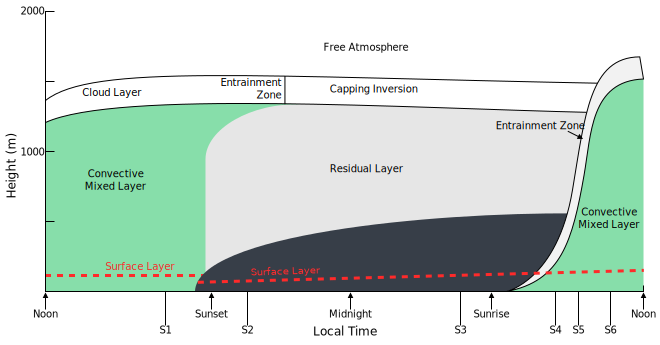
\includegraphics[width=0.8\linewidth]{chapter01/Atmospheric_boundary_layer.pdf}
    \caption{Évolution journalière schématique de la couche limite atmopshèrique.
        Credit: By
        \href{https://commons.wikimedia.org/w/index.php?curid=18862904}{NikNaks} - Own
        work based on:
        \url{http://ars.sciencedirect.com/content/image/1-s2.0-S0360128504000371-gr4.jpg}.
        See also: \url{http://www.archaeocosmology.org/eng/tropospherelayers.htm}., CC
        BY-SA 3.0
    }%
    \label{fig:chapter01/Atmospheric_boundary_layer}
\end{figure}

\section{Les aérosols atmospheriques}%
\label{sec:les_aerosols_atmosphereiques}

\subsection{Qu'est-ce qu'un aérosol ?}%
\label{sub:quest-ce-quun-aerosol}

L'air que nous respirons est constitué majoritairement de gas (\ce{N2}, \ce{O2},…) mais
également de particule solide ou liquide en suspension dans l'air. Ces particules, très
légères et de taille micrométriques ou moins, constituent une famille de composé appellé
communément particule fine, \textit{particulate matter} (PM) ou improprement particule
diesel dans le grand public.

Leur taille varient de quelques nanometres à plusieurs dizaines de micromètres.
À titre de comparaison, cela reviendrait à mettre dans la même catégorie une marche de
\SI{100}{m} pour aller chercher son pain à un voyage de \SI{10000}{km}.
Ainsi, cette nomenclature "PM" regroupe nécessairement des objets aux caractéristiques
très diverses. En effet, comme le montre la Figure~\ref{fig:aerosolDistribution}, selon
que l'on observe les PM en s'intéressant à leur nombre, surface ou volume, l'importance
relative des classes de tailles change complètement.
\begin{figure}[ht]
    \centering
    \includegraphics[width=0.5\textwidth]{aerosolDistribution.pdf}
    \caption{Distribution \textbf{(a)} en nombre, \textbf{(b)} surface, et
        \textbf{(c)} volume, pour un ensemble typique de distribution trimodale
        d'aérosols. Figure adaptée du livre de~\textcite{seinfieldAtmospheric1998}.}
    \label{fig:aerosolDistribution}
\end{figure}

La nomenclature des aérosols est ainsi historiquement fondé sur leur taille:
\begin{itemize}
    \item \PMdix, dont le diamètre aérodynamique inférieur ou égal à \SI{10}{\um}
    \item \PMdc, dont le diamètre aérodynamique inférieur ou égal à \SI{2.5}{\um}
    \item \PMun, dont le diamètre aérodynamique inférieur ou égal à \SI{1}{\um}
\end{itemize}

Ces différents modes reflètes différents procédés conduisant à leur présence dans l'air,
allant de la nucléation à partir de composé gaseux ou de source de combustion pour le mode
dit d'Aikten, le plus fins (prépondérant en nombre), permettant par coagulation
d'atteindre des particules plus grosses (mode d'accumulation) allant jusqu'au \PMdc, pour
enfin, lorsque la vitesse de coagulation est suffisante, atteindre le mode grossier
\PMdix, pouvant également être allimenté par diverse autres sources comme la remise en
suspension par le vent, les pollens, les activités humaines, etc, comme nous le verons
plus loin.

These categories do not have the same
chemical composition nor shape as they reflect different source or different process in
place in the atmosphere. Indeed, aerosols can react with the gas (\ce{SO2},
\ce{NO2}, \ce{NH3} for instance), radiation or radicals (the so call hydroxyl radical
\ce{HO^.}) or even with other aerosols and form new species or bigger aerosols. We then
call this aerosol \emph{secondary aerosol} as it do not reflect a primary source but
reaction in the atmosphere.

\begin{figure}[ht]
    \centering
    \includegraphics[width=1.0\textwidth]{aerosol_micrographs.jpg}
    \caption{Image au microscope electronique à balayage, à des échelles différentes,
        illustrant la diversité de forme des aérosols.
        De gauche à droite : cendre volcanic, polen, sel de mer et suie. Micrographies de
        l'USGS, UMBC (Chere Petty) et de l'Arizona State University (Peter Buseck). Credit
        : NASA earthobservatory
    \url{https://earthobservatory.nasa.gov/Features/Aerosols/}.}
    \label{fig:micrography}
\end{figure}
An aerosol is composed of several chemical species like ions (\SOq, \NOt, \ce{Na+},
\ce{Cl-}, \ce{Mg^2+}, etc), metals (\ce{Cu}, \ce{Al}, \ce{Ti}, \ce{Ca}, etc), and organics species
(cellulose or other sugar, \og black carbon\fg, hopanes, etc).  They come from different
sources: natural like volcano, biology, desert (resuspension due to the wind) or marine
spray for instance and anthropogenic like traffic exhaust, brake wear, industry, biomass
burning or agriculture.  Each of these sources emits different species, in different
quantity and in different place of the atmosphere and of the Earth and with different
shape as shown in fig.~\ref{fig:micrography}.  However, the average lifetime of an aerosol
is from hour to week, and then can impact a wide area.  For instance the black carbon
emitted in developed countries is a major issue for the ice melt in the Artic's iceshelf.
More generally, aerosols are a key parameter in the climate system as they interact with
the Solar and Earth radiation, act as cloud/ice condensation nucleii and sectionicipate to
the precipitation process \autocite{boucherClouds2013}.


\subsection{Impacts climatiques des aérosols}%
\label{sub:impacts_climatiques_des_aerosols}
\paragraph{Noyaux de condensation}%
\label{par:noyaux_de_condensation}

\paragraph{Impact radiatif}%
\label{par:impact_radiatif}



\subsection{Impacts environnementaux}%
\label{sub:impacts_environnementaux}

\paragraph{Transport longue distance}%
\label{par:transport_longue_distance}


\paragraph{Polluants émergents}%
\label{par:polluants_emergents}



\subsection{Impacts sanitaires}%
\label{sub:impacts_sanitaires}



\section{Détermination des sources d'émission des PM}%
\label{sec:source_apportionment_of_pm}

\subsection{Signature chimique des sources d'émissions}%
\label{sec:chemical_signature_of_the_sources}

\subsection{Source apportionment model}%
\label{sec:source_apportionment_model}

\subsubsection{Direct modeling}%
\label{sub:direct_modeling}

\paragraph{Lagrangian or dispersion model}%
\label{sub:lagrangian_or_dispersion_model}

\paragraph{Deterministic chemistry transport model (CTM)}%
\label{sub:deterministic_chemistry_transport_model_ctm_}

\subsubsection{Receptor model}%
\label{sec:receptor_model}

\paragraph{Chemical mass balance (CMB)}%
\label{sub:chemical_mass_balance_cmb_}

\paragraph{Principal component analysis (PCA)}%
\label{sub:principal_component_analysis_pca_}

\paragraph{Positive matrix factorization (PMF)}%
\label{sub:positive_matrix_factorization_pmf_}


\section{Vers une mesure unifiée: le potentiel oxydant}%
\label{sec:le_potentiel_oxydant_des_aerosols}

Devant la grande variété de chimie, forme, taille, etc. des aérosols, il apparaît
compliqué de résumer la toxicité de l'air que l'on respire à sa simple concentration
massique en aérosols. En effet, il est évident que respirer un~\ugm{} de sable n'aura pas
le même impact sur notre santé qu'un~\ugm{} de mercure ou de plomb.
Seulement, la mesure massique est l'une des plus simples a implémenter en routine et est
également facilement automatisable, permettant ainsi un premier ordre de grandeur de 
l'exposition des populations. Aussi, il est important de rappeler que les aérosols n'ont
pas qu'un impacte sanitaire, mais également climatique (voir
section~\ref{sub:impacts_climatiques_des_aerosols}), pour lequel la messure de la concentration est tout a
fait adaptée.

Afin de répondre à ce problème, il a été proposé dans les années 2010 une nouvelle mesure,
intégratrice des propriétés physico-chimique des aérosols, sensé être plus proche des
impacte sanitaire occasioné par les PM. En effet, un des mécanismes suspecté d'être à
l'origine des troubles sanitaires engendrés par les aérosols est le stresse oxydatif
induit lors de l'inhalation des particules, entrainant une cascade de réaction au sain de
notre organisme.
Cette nouvelle mesure tente de quantifier les espèces réactive de l'oxygène (ROS) présente
ou induite par les aérosols en mettant en contact les aérosols et un antioxydant.
Le suivit de la cinétique de la réaction permet ainsi d'estimer la réactivité de la
particule, prenant en compte non seulement sa chimie, mais aussi la taille et forme des
particules à travers leurs surface de réaction et également les potentiels "effet
cocktail" lors de la combinaison de différentes espèces chimiques.

\subsection{Methodologie de mesure}%
\label{sub:methodologie_de_mesure}

\subsubsection{Prendre en compte la bioaccessibilité: SLF}%
\label{sub:prendre_en_compte_la_bioaccessibilite_slf}

\subsubsection{Differents agent réactant}%
\label{ssub:differents_agent_reactant}

\paragraph{Mesure par Ditiothreitol}%
\label{ssub:mesure_par_ditiothreitol}

\paragraph{Mesure par Acide ascorbic}%
\label{ssub:mesure_par_acide_ascorbic}

\paragraph{Mesure par DCFH}%
\label{ssub:mesure_par_dcfh}

\paragraph{Autres methodes de mesure}%
\label{sub:autres_methodes_de_mesure}

\subsubsection{Unitées de mesures}%
\label{ssub:unitees_de_mesures}

Mesure de réactivité par ug de PM ou par m3 d'air respirer.

\subsection{État de la connaissance du PO}%
\label{sub:etat_de_la_connaissance_du_po}



\addcontentsline{toc}{section}{Bibliography}
\printbibliography[segment=2,heading=subbibliography]


\chapter{Approfondissement des connaissances des sources des PM}%
\label{cha:approfondissement_des_connaissances_des_sources_des_pm}
\PartialToc
\clearpage
\section*{Introduction}%
\label{sec:introduction}
\addcontentsline{toc}{section}{Introduction}


Les travaux présentés dans ce chapitre ont été menés afin d'approfondir les connaissances
des processus d'émissions de différents composés des PM. En effet, le modèle PMF utilisé
pour tracer l'origine des sources d'aérosol nécessite une base de connaissance préalable à
son utilisation car comme nous l'avons vu, plusieurs paramètres doivent être choisis par
l'expérimentateur, notamment les variables servant d'entrainement au modèle.

Un modèle étant nécessairement une représentation simplifiée de la réalité, il convient de
trouver le bon équilibre entre un modèle trop complexe, qui serait difficilement
interprétable, et un modèle trop simple, qui n'apporterait pas de nouvelles informations.
Le cas de la PMF, et le \textit{machine learning} en général, n'échappe pas à cette règle.
Il faut en effet choisir soigneusement les variables d'entrée du modèle pour lui permettre
d'extraire des informations géochimiquement pertinentes d'un ensemble de donnée. Cela se
traduit par la détermination d'espèce traceuse de processus d'émissions ou de
transformations dans l'atmosphère, puis de leur utilisation conjointe dans le modèle PMF,
permettant alors d'isoler de nouveaux facteurs et de raffiner la contribution des autres
espèces aux facteurs restants.

Aussi, un modèle procède toujours à une étape de validation. Dans notre cas, nous n'avons
pas de référence pouvant servir de témoin positif. Nous pouvons cependant nous servir de
2 procédés : 1) la confrontations à d'autres méthodes de \textit{sources-apportionment},
indépendantes de la PMF (carbone 14 (\textcite{bonvalotEstimating2016} et
\textcite{chevrierChauffage2016}), Aethalometre, etc) ou 2) estimer la fiabilité des
résultats PMF par cohérence géophysique, par exemple en retrouvant l'origine géographique
des sources d'émissions.

Les travaux de cette thèse ont ainsi conduit à différents développements ou applications
méthodologiques et techniques.
\begin{enumerate}
    \item Nous verrons dans un premier temps que l'origine géographique des masses d'air
        par méthode PSCF a permis de consolider les solutions obtenues par méthodologie
        PMF, mais a également apportée une vision nouvelle de la provenance du MSA,
        supposé jusqu'alors d'origine exclusivement marine~\autocite{gollyOrganic2019}.
    \item Dans un second temps, nous expliquerons en quoi le recensement et
        l'harmonisation de la base de donnée de filtre de prélèvement ambiant a été
        utilisé afin de généraliser des observations à un ensemble de 28 sites de
        mesures et a conduit à la quantification des processus d'émissions biogéniques
        primaires~\autocite{samakePolyols2019,samakeArabitol2019}.
    \item Enfin, nous présenterons un travail en cours sur la variabilité fine échelle
        des sources de PM et l'importances des facteurs d'oxydations secondaires,
        identifiés par l'ajout de nouveaux traceurs organiques dans la
        PMF~\autocite{borlazaSourceinprep}.
\end{enumerate}
\todo{Et INACS dans tout ca ?}


\section{Provenance géographique des composés chimiques et facteurs}%
\label{sec:provenance_géographique_des_composés_chimiques_et_facteurs}

Pour déterminer l'origine des sources des composés chimiques retrouvé à un site récepteur,
il est possible de retracer sa provenance géographique. Nous verrons d'abord le cas simple
de la rose des polluants, avant d'expliciter plus en avant la méthode PSCF.

\subsection{Cas simple : la rose des polluants}%
\label{sub:cas_simple_la_rose_des_polluants}

L'un des moyens les plus simples pour cela est de coupler des mesures de direction et
vitesse de vent et d'établir une rose des polluants. J'ai pu utiliser ce procédé à des
fins exploratoires lors de ma thèse, ce qui m'a conduit à contribuer au développement du
package python
\href{https://github.com/python-windrose/windrose/}{windrose}~\autocite{scls19frPythonwindrose2019}.
Cependant, cette méthode n'est utile que pour la détermination de source proche du site
récepteur car dès lors que l'on s'en éloigne, l'orientation et vitesse des vents varient
et l'hypothèse de déplacement uniforme de la masse d'air est invalidée.  Or, il est
courant que les aérosols proviennent de sources non locales, limitant l'utilisabilité de
cette méthode.

En revanche, il est possible d'utiliser les rétrotrajectoires complètes des masses d'air
pour remonter aux sources géographiques potentielles et également de coupler ces
trajectoires à des informations physico-chimiques comme la concentration en polluants
observés sur le site récepteur, la présence de pluie déposant les aérosols par dépôt
humide ou encore la hauteur de la masse d'air.

\subsection{Prendre en compte l'histoire de la masse d'air : PSCF}%
\label{sub:prendre_en_compte_l_histoire_de_la_masse_d_air_PSCF}

\subsubsection{Méthodologie}%
\label{ssub:méthodologie}

L'une des méthodes les plus largement utilisée dans la littérature est la \textit{Potential
source contribution function} (PSCF), permettant de combiner des ensembles de trajectoires à
des modèles récepteurs. Le principe consiste à calculer les rétrotrajectoires d'un site
récepteur donné et d'associer à chacune d'elle la concentration du polluant ou de la
source considéré le jour de son passage au niveau du site récepteur. En discrétisant les
trajectoires en 1 point toutes les X minutes ou heures et en appliquant une grille
régionale, il est alors possible de dénombrer combien de rétrotrajectoires sont passés par
chacune des grilles.  Le ratio du nombre de trajectoire associée à une forte concentration
aux coordonnées $i$, $j$, noté $m_{ij}$, par le nombre total de trajectoire étant passé
par ces coordonnés notées $n_{ij}$, nous donne une probabilité de provenance géographique
de ce composé ou source pour les coordonnées $i$, $j$, noté $PSCF_{ij}$ :
\begin{align}
    \label{eq:PSCF}
    PSCF_{ij} &= \frac{m_{ij}}{n_{ij}}.
\end{align}

Des améliorations ont été apportées à cette méthode afin de prendre en compte les cellules
ayant un faible pourcentage de passage de rétrotrajectoires, augmentant artificiellement
le ratio $\frac{M}{N}$. Une manière de contrebalancer ce biais et d'ajouter une fonction
poids, dépendant de la fréquence de passage des rétrotrajectoires sur chacune des
cellules. Dans la figure~\ref{fig:chapter02/PSCF_method}, illustrant la PSCF, on voit que
la cellule où 2 rétrotrajectoires sont passés se voit attribuer la même probabilité que
celles avoisinantes, où seule une rétrotrajectoire a résidé. Or, il serait plus pertinent
d'avoir une probabilité plus forte pour cette cellule, indiquant que chaque
rétrotrajectoire ayant résidé à ces coordonnées est riche du composé suivit.  Différentes
fonctions poids existent, le plus souvent présentant différents seuils en fonction du
nombre de rétrotrajectoires par cellule~\autocite{bressiSources2014,petitSources2019}.

Aussi, pour avoir une représentativité statistique suffisante des sources potentielles, il
est nécessaire de calculer un grand nombre de rétrotajectoire, correspondant à chacun des
jours de prélèvement sur le site récepteur.


\begin{figure}[ht]
    \centering
    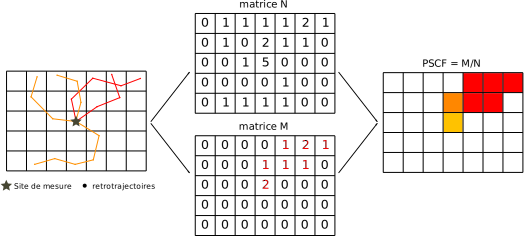
\includegraphics[width=0.9\linewidth]{chapter02/PSCF_method.pdf}
    \caption{Illustration de la méthode PSCF : les rétrotrajectoires depuis le site de
        mesure sont calculées, celles associées à une concentration seuil sont
        représentées en rouge, les autres en orange. Les matrices N et M s'obtiennent par
        simple décompte du nombre de rétrotrajectoires passés dans chaque cellule de
        taille prédéfinies, puis le ratio nous donne une estimation de l'origine
    géographique, représentée ici terme d'intensité de rouge.}%
    \label{fig:chapter02/PSCF_method}
\end{figure}

\subsubsection{Automatisation et simplification : pyPSCF}%
\label{ssub:automatisation_et_simplification_pypscf}

Ces étapes fastidieuses de calcul des rétrotrajectoires et de PSCF ont été automatisés
dans un paquet python, pyPSCF\footnote{Dépot git pyPSCF:
\url{https://gricad-gitlab.univ-grenoble-alpes.fr/webersa/pyPSCF}}, permettant le
traitement d'un grand nombre de rétrotrajectoire en utilisant le modèle lagrangian
HYSPLIT et calculant de manière facilité une PSCF en un site donné, en variant notamment
les différents paramètres succeptibles d'influencer le modèle.

\subsection{Application : Importance et origine géographique du MSA ? (Golly et al. 2019)}%
\label{sub:origine_terrestre_ou_marine_du_msa_}

Comme expliqué précemment, une part importante des aérosols provient de sources
secondaires, c'est-à-dire du vieillissement et des réactions dans l'atmosphère. Une part
importante de ces aérosols secondaires sont d'origines organiques. Les travaux
de~\textcite{gollyOrganic2019}, auxquels j'ai pris part, s'attachent notamment à la
quantification de cette matière organique secondaire, sur 5 sites ruraux en France
pendant l'année 2013, par la mesure de deux espèces issues de processus secondaires : le
MSA et l'oxalate.  Nous avons pu montrer que le MSA, considéré comme provenant de
l'oxydation du DMS, peut contribuer jusqu'à 10 à 20\% de l'OC en période chaude,
indiquant une forte proportion d'aérosols organiques secondaires durant l'été. Mais
surtout, le MSA est considéré comme provenant des émissions de DMS du phytoplanction
marin, au point qu'il est proposé comme méthode de séparation entre le sulfate d'origine
marine et ses autres provenances.

En conduisant une analyses PSCF sur les 25\% des jours les plus fortement chargés en MSA,
nous avons pu confirmer l'importance marine de ce composé, mais également montrer qu'une
part non négligeable semble provenir d'environnement terrigène (voir
figure~\ref{fig:chapter02/golly_PSCF_MSA}), confortant les études suggérants des
processus d'émissions du MSA par des sources biologiques
terrestres~\autocite{bozzettiArgon2017}, pouvant provenir des forêts ou des
sols~\autocite{jardineDimethyl2015,miyazakiSeasonal2012}.

L'une des implications directes de ces travaux résulte en l'ajout systématique du MSA
comme variable d'entrée des études PMF, quelque soit leur localisation. En effet, le
signal du MSA est clairement distinct des autres espèces chimiques mesurées et représente
également une part important de la matière organique. Cette espèce est donc a minima
traceuse de processus secondaires présent sur l'ensemble de l'europe occidental.

\begin{figure}[ht]
    \centering
    \includegraphics[width=0.9\linewidth]{chapter02/golly_PSCF_MSA.png}
    \caption{Probabilité de l'origine géographique du MSA, issue de l'article
        de~\textcite{gollyOrganic2019}. Bien que l'on retrouve l'origine marine du MSA,
        les sites de Dieulefit, OPE ou Peyrusse-Vieille indiquent également une forte
        probabilité d'origine terrestre de ce composé.}%
    \label{fig:chapter02/golly_PSCF_MSA}
\end{figure}

\subsection{Application 2 : Validation des solutions PMF}%
\label{sub:application_2_validation_des_solutions_pmf}

Une autre utilisation de la PSCF consite à croiser les informations issues de la PSCF et
des PMF.
En effet, il n'existe pas de moyen simple de valider le sens géochimique d'une solution
PMF autrement que l'expertise et les connaissances de l'utilisateur.
Une fois une solution obtenu, il est possible de conduire une étude PSCF sur les
différents facteurs identifiés par la PMF. Ainsi, on s'attend à ce que le facteur
\textit{sel de mer} provienne géographiquement d'un océan ou d'une mer. De même la
\textit{combustion de biomasse domestique} ne devrait pas pointer d'emplacement
particulier puisqu'il s'agit d'une source diffuse.

\todo{Exemple de l'OPE : sel de mer et combustion de biomass}


\section{Généralisation d'observations}%
\label{sec:généralisation_dobservations}

\subsection{Mise en place d'une base de donnée harmonisée}%
\label{sub:mise_en_place_d_une_base_de_donnée_harmonisée}

\subsection{Application : Importance des émissions primaires biogéniques (Samaké et al.
2019)}%

\label{sub:application_importance_des_émissions_primaires_biogéniques_samaké_et_al_2019_}


\section{De nouveaux traceurs secondaires pour les PMF ?}%
\label{sec:amélioration_des_solutions_pmf_grâce_à_de_nouveaux_traceurs_organiques}

\subsection{Problématique}%
\label{sub:problématique}

\subsection{Ajout des acides organiques comme traceur du SOA ? (Borlaza et al. in prep)}%
\label{sub:ajout_des_acides_organiques_comme_traceur_du_soa_borlaza_et_al_in_prep_}




\printbibliography[segment=\therefsegment,heading=subbibliography]



\chapter{Développent méthodologique d'attribution des sources de PM}
\label{cha:developpement_methodologique_dattribution_des_sources_de_PM}
\PartialToc
\clearpage
\input{chapters/chapter03_developpement.tex}

\chapter{Méthodologie de déconvolution des sources de PO}
\label{cha:methodology_for_the_attribution_of_intrisinc_op_to_a_pm_source}
\PartialToc
\clearpage
\input{chapters/chapter03.tex}

\chapter{Passage à l'échelle régionale : application à 15 sites d'étude en France}
\label{cha:application_to_15_sites_in_France}
\PartialToc
\clearpage
\input{chapters/chapter04.tex}

\chapter{Vers une modélisation spatialisé du PO}
\label{cha:spatio_temporal_modelizing}
\PartialToc
\clearpage

\section{Generalization of observations}%
\label{sec:generalization_of_observation}

\subsection{Representativness of ground-based sources-apportionment in France}%
\label{sub:representativness_of_ground_based_sources_apportionment_in_france}


\subsection{Representativness of intrinsic OP per PMF profile in France}%
\label{sub:representativness_of_intrinsic_op_per_pmf_profile_in_france}



\section{Implementation in chemistry transport model}%
\label{sec:implementation_in_chemistry_transport_model}

Lotos euros



% =====================================================================================
% Bibliographie complète {{{
% \addcontentsline{toc}{part}{Bibliography}
% \printbibheading
\printbibliography
% \bibbysegment[heading=subbibliography]

% }}}
% =====================================================================================

% =====================================================================================
% Appendix {{{
\addcontentsline{toc}{part}{Appendix}
\appendix
\setcounter{table}{0}
\setcounter{figure}{0}
\setcounter{equation}{0}
\renewcommand{\thetable}{\thesection-\arabic{table}}
\renewcommand{\thefigure}{\thesection-\arabic{figure}}
\renewcommand{\theequation}{\thesection-\arabic{equation}}
% }}}
% =====================================================================================
\end{document}
